\section{SW 2 Detection Theory}
When one transmits data over a non ideal channel, the output data is not the same anymore, which means the data could look completely different.  But to still reconstruct the correct data a detection algorithm on the output of the channel is needed to decide which data was originally sent. This page will have a look into this detection algorithm and how one can calculate how big the probability is that our detection algorithm is wrong.
\section{Additive White Gaussian Noise (AWGN)}
When we transmit a signal over a channel it is most probably that AWGN is added to our signal because we have thermal noise in our channel.
\subsection{Thermal noise}
Thermal noise occurs due to the vibration of charge carriers within an electrical conductor and is directly proportional to the temperature, regardless of the applied voltage.
AWGN ($n(t)$) which is also called a normal distribution, Gaussian or Gauss distribution with a mean ($\mu$) of zero and a variance of $\sigma^2$ can be described with the following probability density function:
\begin{equation}\label{eq:gauss_distribution_white noise}
p(n)=\frac{1}{\sigma \sqrt{2 \pi}} e^{-n^2 / 2 \sigma^2}
\end{equation}
\begin{equation}\label{eq:gauss_distribution}
p(x)=\frac{1}{\sigma \sqrt{2 \pi}} e^{-\frac{1}{2}(\frac{x-\mu}{\sigma})^2}
\end{equation}
The function says that the probability is very high, that we measure a signal that has a value close to zero ($n(t)$ has zero mean) and very low that we measure a value that is very far away from zero. 
\subsection{Probability}
The probability that we measure a certain value can be calculating by integrating the Gaussian function. But for this it is important to know that the cumulative distribution function (\href{https://en.wikipedia.org/wiki/Cumulative_distribution_function}{CDF}) of the standard normal distribution, usually denoted with the capital Greek letter $\Phi$ is not \href{https://en.wikipedia.org/wiki/Elementary_function}{elementary}, which means it's integral can not be described with a normal function. Therefore, often the \href{https://en.wikipedia.org/wiki/Q-function#Bounds_and_approximations}{Q-Function} is used to calculate the probability (a certain area below the function/ the integral with defined boundaries). Note that the q-function is the probability that a normal (Gaussian) random variable will obtain a value larger than $x$ standard deviations. The value of Q(x) can normally be looked up in tables, whereas gaussian distribution functions with a mean other than zero and a variance different from one can be not.
$$
Q(x)=\frac{1}{\sqrt{2 \pi}} \int_x^{\infty} \exp \left(-\frac{u^2}{2}\right) d u
$$
\begin{figure}[ht]
  \centering
  \resizebox{10cm}{!}{\subimport{images/}{probability1.tex}}
  %\includestandalone[width=1\linewidth]{wiener3.tex} % without the `.tex` extension
  \caption{Probability}
  \label{fig:probability1}
\end{figure}
Furthermore white noise is uncorrelated which means the autocorrelation plot is a dirac function.
\subsection{Bayes Law}
To calculate the BER or SER it is important to understand Bayes Law. Therefore, one finds an introduction to it in this section.
\begin{equation}
p(B) p(A \mid B)=p(B \mid A) p(A)
\end{equation}
Or in our application:
\begin{equation} \label{eq:map_1}
p\left(s_i \mid z\right)=\frac{\textcolor{blue}{p\left(z \mid s_i\right)} \textcolor{olive}{p\left(s_i\right)}}{\textcolor{violet}{p(z)}}
\end{equation}
\begin{itemize}
\item $\textcolor{olive}{p\left(s_i\right)\text{ a priori probability}}$
\item $\textcolor{blue}{p\left(z \mid s_i\right)\text{conditional probability or Likelihood}}$
\item $\textcolor{violet}{{p(z)}\text{ a poster priori probability}}$
\end{itemize}
\subsubsection{priori information}
$p(s_i)$ is the "a priori" probability that $s_i$ is sent. It is a feature of the data and not of the transmission, furthermore it is not always known. \newline
When one has this probability, it can be used to make a decision. For example, when we transmit language, the probability of sending a "q" is very low, but the probability of sending an "i" is much higher.

$\textcolor{blue}{p\left(z \mid s_i\right)}$, is a conditional probability: the probability of event z occurring given that $s_i$ is true. It is also called the posterior probability of z given $s_i$. In words, it says when we send signal $s_i$ the probability is $\textcolor{blue}{p\left(z \mid s_i\right)}$ to receive z. 
\subsubsection{Example}
10\% of the accidents is caused by drunk drivers $P(drunk \mid acc)=0.1$, The rest of the accident is caused by not drunk drivers $P(sober \mid acc)=0.9$ Which says ten precent of the accidents is cause by drunk drivers and 90\% of the accidents is caused by sober drivers, which could lead to the conclusion that one should be drunk when driving a car. Which is actually not true. Lets further assume that the probability of making an accident is $p(\operatorname{accident})=10^{-6}$ and the probability of being drunk is $p(drunk)=0.1$ and of being sober is $p(drunk)=0.9$. With bayes law we can now calculate what the probability of having an accident while being drunk is.

$$
p\left(\operatorname{accident} \mid p(drunk)\right)=\frac{p\left(p(drunk)\mid \text { accident }\right) \cdot p(\operatorname{accident})}{p(drunk)}=\frac{10^{-1} \cdot 10^{-6}}{10^{-2}}=10^{-5}
$$
$$
p\left(\operatorname{accident} \mid p(sober)\right)=\frac{p\left(p(sober)\mid \text { accident }\right) \cdot p(\operatorname{accident})}{p(sober)}=\frac{0.9 \cdot 10^{-6}}{0.99}\approx 10^{-6}
$$

\subsubsection{MAP receiver (Considers probability)} 
$$
\frac{p\left(\boldsymbol{r} \mid H_1\right)}{p\left(\boldsymbol{r} \mid H_0\right)}\underset{\substack{H_0}}{\stackrel{H_1}{\gtrless}} \frac{P_0}{P_1}
$$
This is also what one can see in \autoref{fig:probability_9}.
\begin{itemize}
\item Maximizes "a posteriori" probability
\item Choose $s_i$ such that $p(s_i \mid z)$ is maximized(see equation \ref{eq:map_1}), for this $\textcolor{olive}{p\left(s_i\right)}$ must be known
\end{itemize}
\subsubsection{ML(Maximum Likelihood) receiver (Does not consider probability)} 
Is the same as the MAP but maximizes only $\textcolor{blue}{p\left(z \mid s_i\right)}$. When $\textcolor{olive}{p\left(s_i\right)}=1/M$ ML and MAP are the same. \newline
To sum it up, what we generally do is we look at the point we measured which probability density function has the higher probability or to which point we are closer. The integral under the curve to the point also gives us the probability that our assumption was wrong.
\begin{figure}[ht]
  \centering
  \resizebox{10cm}{!}{\subimport{images/}{probability2.tex}}
  \caption{Probability2}
  \label{fig:probability_2}
\end{figure}
\section{Bit-error rate BER}
There are different ways to find out the error rates: (When confused about SER and BER watch the following  \href{https://youtu.be/du-sExIUV-Y}{video})
\begin{itemize}
\item Build the system and measure it $\Rightarrow$ this method is very time consuming and one has to build the real system
\item Monte-Carlo simulations $\Rightarrow$ this is even more time consuming, since the simulation is normally not as fast as the real application.
\item Analytic (numerical) solution $\Rightarrow$ this is very difficult to solve in certain cases
\end{itemize}

\subsubsection{Exercise Binary maximum-likelihood and MAP detection}
A random variable $X$ takes on the values 0 and 1 with the probabilities $P(X=0)=0.2$ and $P(X=1)=0.8$. A second random variable $Y$ has a Gaussian probability density function with mean $m=0$ and standard deviation $\sigma=1$. Our observation is the sum $Z=X+Y$.
\begin{enumerate}
    \item Determine and draw $p(z \mid X=0)$ and $p(z \mid X=1)$.\newline
    When X is zero Z must be Y, and therefore $p(z \mid X=0)=\frac{1}{\sqrt{ } 2 \pi} e^{-\frac{z^2}{2}}$. When X is one Z is 1+Y and therefore $p(z \mid X=1)=\frac{1}{\sqrt{2 \pi}} e^{-\frac{(z-1)^2}{2}}$
    \begin{figure}[ht]
      \centering
      \resizebox{8cm}{!}{\subimport{images/}{probability9.tex}}
      \caption{Probability9}
      \label{fig:probability_9}
    \end{figure}
    \item Use the maximum $a$-posteriori detection (MAP) to decide on the value of $X$, if $z=0.1$ was observed.\newline
    From \autoref{eq:gauss_distribution} one knows that $p(x)=\frac{1}{\sigma \sqrt{2 \pi}} e^{-\frac{1}{2}(\frac{x-\mu}{\sigma})^2}=\frac{1}{1 \sqrt{2 \pi}} e^{-\frac{1}{2}(\frac{0.1-0}{1})^2}$

    $$
    \begin{aligned}
    & X=0 \quad \Rightarrow \quad p(0.1 \mid X=0) \cdot P(X=0)=\frac{1}{\sqrt{2 \pi}} e^{-\frac{0.1^2}{2}} \cdot 0.2 \approx 0.079 \\
    & X=1 \quad \Rightarrow \quad p(0.1 \mid X=1) \cdot P(X=1)=\frac{1}{\sqrt{2 \pi}} e^{-\frac{(0.1-1)^2}{2}} \cdot 0.8 \approx 0.213
    \end{aligned}
    $$
    \begin{figure}[ht]
      \centering
      \resizebox{8cm}{!}{\subimport{images/}{probability10.tex}}
      \caption{Probability10}
      \label{fig:probability_10}
    \end{figure}
    Therefore we would decide for X=1 (this probability was higher)
    \item What would the decision be if you used maximum likelihood detection (ML)?\newline
    $$
    \begin{aligned}
    & X=0 \quad \Rightarrow \quad p(0.1 \mid X=0)=\frac{1}{\sqrt{2 \pi}} e^{-\frac{0.1^2}{2}} \approx 0.397 \\
    & X=1 \quad \Rightarrow \quad p(0.1 \mid X=1)=\frac{1}{\sqrt{2 \pi}} e^{-\frac{(0.1-1)^2}{2}} \approx 0.266
    \end{aligned}
    $$
    Therefore one would decide for X=0.
    \item Below which threshold of the observation value $z$ should you decide in favor of $X=0$ using MAP detection?\newline
    $$
    \begin{aligned}
    p(z \mid X=0) \cdot P(X=0) & >p(z \mid X=1) \cdot P(X=1) \\
    \frac{1}{\sqrt{2 \pi}} e^{-\frac{z^2}{2}} \cdot 0.2 & >\frac{1}{\sqrt{2 \pi}} e^{-\frac{(z-1)^2}{2}} \cdot 0.8 \\
    \frac{e^{-\frac{z^2}{2}}}{e^{-\frac{(z-1)^2}{2}}} & >\frac{0.8}{0.2} \\
    e^{-\frac{2 z-1}{2}} & >4 \\
    \frac{1-2 z}{2} & >\ln (4) \\
    z & <\frac{1}{2}-\ln (4)=-0.886
    \end{aligned}
    $$
    This is also what one can see in \autoref{fig:probability_10}.
    \item Below which threshold of the observation value $z$ should you decide in favor of $X=0$ using ML detection?\newline
    $$
    \begin{aligned}
    p(z \mid X=0) & >p(z \mid X=1) \\
    \frac{1}{\sqrt{2 \pi}} e^{-\frac{z^2}{2}} & >\frac{1}{\sqrt{2 \pi}} e^{-\frac{(z-1)^2}{2}} \\
    \frac{e^{-\frac{z^2}{2}}}{e^{-\frac{(z-1)^2}{2}}} & >1 \\
    e^{-\frac{2 z-1}{2}} & >1 \\
    \frac{1-2 z}{2} & >0 \\
    z & <\frac{1}{2}
    \end{aligned}
    $$
    This is also what one can see in \autoref{fig:probability_9}.
\end{enumerate}



\subsection{Analytic Solution}
To get the BER in an analytical way, we must know the following. White noise has a Gaussian distribution, as mentioned above, which can be described in with the formulat mentioned in equation \ref{eq:gaussian}. The signal which we measure is a \href{https://en.wikipedia.org/wiki/Energy_(signal_processing)}{discrete time signal} which energy is given by equation \ref{eq:energy_discrete_time}.
\begin{equation} \label{eq:gaussian}
f(x)=\frac{1}{\sigma \sqrt{2 \pi}} e^{-\frac{1}{2}\left(\frac{x-\mu}{\sigma}\right)^2}
\end{equation}
\begin{equation} \label{eq:energy_discrete_time}
E_s=\langle x(n), x(n)\rangle=\sum_{n=-\infty}^{\infty}|x(n)|^2
\end{equation}
\subsubsection{BPSK}
When we use the equations above, we can calculate the BER for the BPSK signal. The amplitude of the original signal is $\sqrt{E_s}$ which is a constant. When we add white noise to our signal(which is a constant) the white noise gets shifted, which means $\mu$ the mean is not zero any more but $\sqrt{E_s}$ (The expected value when we do a measurement is now $\sqrt{E_s}$). Therefore the BER which is for binary signals the same as the symbol error rate (SER). Blow one can see the calculation of the probability of error also BER.
$$
\begin{aligned}
P_E &=\int_0^{\infty} p(x \mid s=-1) d x \\
&=\int_0^{\infty} \frac{1}{\sqrt{2 \pi} \sigma} \mathrm{e}^{-\frac{\left(x+\sqrt{E_S}\right)^2}{2 \sigma^2}} d x \\
&=\int_0^{\infty} \frac{1}{\sqrt{2 \pi} \sqrt{\frac{N_0}{2}}} \mathrm{e}^{-\frac{\left(x+\sqrt{E_S}\right)^2}{N_0}} d x \\
&=\int_{\sqrt{E_S}}^{\infty} \frac{1}{\sqrt{2 \pi} \sqrt{\frac{N_0}{2}}} \mathrm{e}^{-\frac{x^2}{N_0}} d x \\
&=Q\left(\sqrt{\frac{2 E_S}{N_0}}\right) .
\end{aligned}
$$
Which corresponds to the blue area in \autoref{fig:probability_3}.
\begin{figure}[ht]
  \centering
  \resizebox{10cm}{!}{\subimport{images/}{probability3.tex}}
  \caption{Probability3}
  \label{fig:probability_3}
\end{figure}
Furthermore the SNR(Signal to noise ratio) for BPSK is $\frac{E_s}{N_0}$, where $N_0$ is the energy of the white noise.
% <iframe src="https://www.youtube.com/embed/vtJ6mAy3xMc" title="YouTube video player" allow="accelerometer; autoplay; clipboard-write; encrypted-media; gyroscope; picture-in-picture" allowfullscreen="" width="560" height="315" frameborder="0"></iframe>
\subsubsection{QPSK}
To calculate the SER of QPSK it is important to know the following:
$$\cos(\ang{45})=\frac{1}{\sqrt{2}}$$
When we assume the the energy per bit is still $E_s$ the distance between two signals is in QPSK $\frac{\sqrt{E_s}}{\sqrt{2}}$ Due to that the probability that we measure a signal on the right side of the $x$-axis when we have sent the signal on the top right corner is $P\left(x>0 \mid s_0\right)$ ,which is given by the formula below. (The factor of two cancels out)
$$
P\left(x>0 \mid s_0\right)=1-Q\left(\sqrt{\frac{E_s}{N_0}}\right)
$$
This is the same probability as $P\left(y>0 \mid s_0\right)$, therefore the probability that we measure the correct signal is $P\left(x>0 \mid s_0\right) \cdot P\left(y>0 \mid s_0\right)= \left(1-Q\left(\sqrt{\frac{E_s}{N_0}}\right)\right)^2$ and therefore the SER is given by the following equation:
\begin{equation}\label{eq:symbol_error_rate_qpsk}
\mathrm{SER}=1-\left(1-Q\left(\sqrt{\frac{E_s}{N_0}}\right)\right)^2
\end{equation}
\begin{figure}[ht]
  \centering
  \resizebox{10cm}{!}{\subimport{images/}{probability4.tex}}
  \caption{Probability4}
  \label{fig:probability_4}
\end{figure}
\subsubsection{Exercise error Probability of QPSK}
\begin{enumerate}
    \item Derive the expression for the SER/BER of a QPSK signal. Hint: Assume the probability for an error in x or y direction to be independent.\newline
    From \autoref{eq:symbol_error_rate_qpsk} one knows that it is for QPSK $\mathrm{SER}=1-\left(1-Q\left(\sqrt{\frac{E_s}{N_0}}\right)\right)^2$. \newline But the derivation would be quite easy. The energy per symbol must be one. Therefore, the amplitude in x and y direction is $\frac{1}{\sqrt{2}}$ since $\sqrt{(\frac{1}{\sqrt{2}})^2+(\frac{1}{\sqrt{2}})^2}=1$ The probability that one makes an error of $p_a$ as it can be seen in \autoref{fig:qpsk_bit_error} is therefore defined as the following.
    $$
    p_a=P\left(x<0 \mid d_0\right) P\left(y>0 \mid d_0\right)=Q\left(\sqrt{\frac{E_s}{N_0}}\right)\left(1-Q\left(\sqrt{\frac{E_s}{N_0}}\right)\right)=Q\left(\sqrt{\frac{E_s}{N_0}}\right)-Q\left(\sqrt{\frac{E_s}{N_0}}\right)^2
    $$
    Since $P\left(x<0 \mid d_0\right)=Q\left(\sqrt{\frac{E_s}{N_0}}\right)$ and $p_b$ as the following:
    $$
    p_b=P\left(x<0 \mid d_0\right) P\left(y<0 \mid d_0\right)=\left(Q\left(\sqrt{\frac{E_s}{N_0}}\right)\right)^2
    $$
    $$
    \begin{aligned}
    \mathrm{BER}_{\mathrm{conv}} & =\frac{1}{2}\left(p_a \cdot(1+2)+p_b \cdot 1\right) \\
    \mathrm{BER}_{\mathrm{Gray}} & =\frac{1}{2}\left(p_a \cdot(1+1)+p_b \cdot 2\right)
    \end{aligned}
    $$
    \begin{figure}[ht]
      \centering
      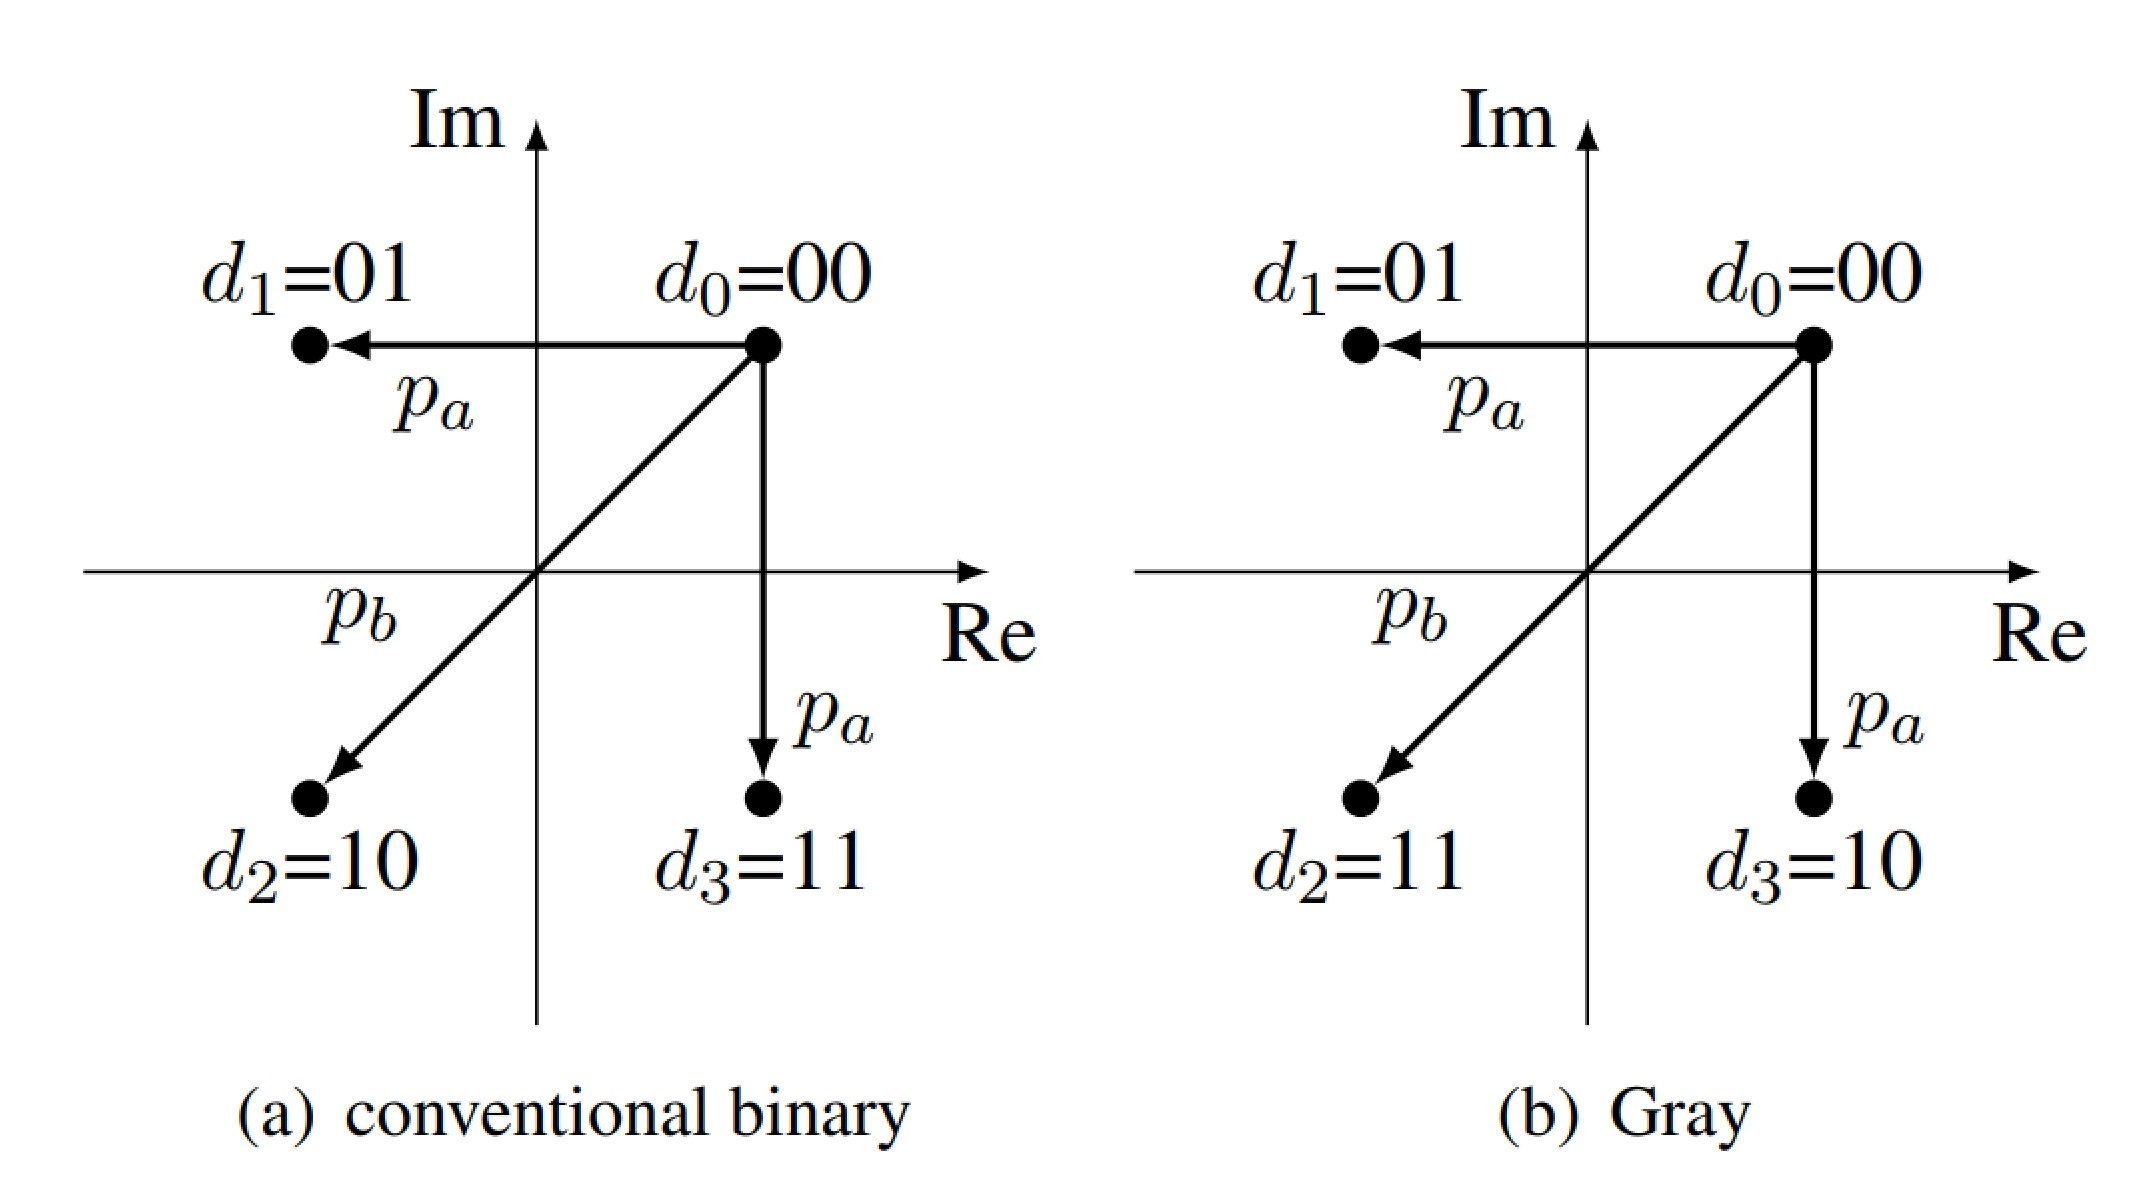
\includegraphics[width=10cm]{images/bit_error.jpg}
      \caption{Error}
      \label{fig:qpsk_bit_error}
    \end{figure}
    \item What difference in BER do we have between Gray code and conventional binary code?\newline
    $$
    \frac{\mathrm{BER}_{\text {conv }}}{\mathrm{BER}_{\mathrm{Gray}}}=\frac{3 p_a+p_b}{2 p_a+2 p_b}=\frac{3 Q(.)-3 Q^2(.)+Q^2(.)}{2 Q(.)-2 Q^2(.)+2 Q^2(.)}=\frac{3-2 Q(.)}{2}
    $$
    For larger $\frac{E_s}{N_0}, Q(\cdot)$ becomes small and can be neglected, leading to
    $$
    \frac{\mathrm{BER}_{\text {conv }}}{\mathrm{BER}_{\mathrm{Gray}}} \approx \frac{3}{2} .
    $$
\end{enumerate}


\section{Signal Space}
A signal space is a vector space with finite dimension. The vectors $\left\{\psi_1(t), \psi_2(t), \ldots \psi_N(t)\right\}$ are orthagonal when the inner products between two different vectors is zero and with the same vector one. $\left\langle\psi_i(t), \psi_j(t)\right\rangle$ stands for the inner product of $psi_i(t)$ and $\psi_j(t)$.
$$
\begin{aligned}
&\left\{\psi_1(t), \psi_2(t), \ldots \psi_N(t)\right\} \\
&\left\langle\psi_i(t), \psi_j(t)\right\rangle= \begin{cases}1 & j=i \\
0 & j \neq i\end{cases}
\end{aligned}
$$
A signal vector is:
$$
s_i(t)=\sum_{j=1}^N a_{i, j} \psi_j(t)
$$
with
\begin{itemize}
\item $a_{i j}$ are the coefficients of $s_i(t)$ in signal space
\item $\underline{S}_i=\left[\begin{array}{ll}a_{i 1} & a_{i 2} \cdots a_{i N}\end{array}\right]$
\item $a_{i k}=\left\langle s_i(t), \psi_k(t)\right\rangle$
\item $\left\|s_i(t)\right\|^2=\sum_{j=1}^N a_{i j}^2$
\end{itemize}
To determine how efficient our protocol is one can calculate the average energy per symbol as below.
$$
E_s=\frac{1}{M} \sum_{i=1}^M\left\|s_i(t)\right\|^2
$$
\begin{itemize}
\item Transmitted signal $s_i(t)$
\item AWGN noise $\hat{n}(t)$
\item threshold $\gamma$
\item Received signal $r(t) = s_i(t) + \hat{n}(t)$
\item Filter output: $z(t)=r(t)*h(t)=s_i(t)*h(t)+\hat{n}(t)*h(t)=a_i(t)+n(t)$
\end{itemize}
$z(t)$ was at any point in time whereas $z(T)$ is at a specific sample point, when we sample once per symbol time T is the symbol time.
The last box in the plot above is the test statistic, dependent of the value of z it will say the signal is one or zero.\newline
When one sends symbol zero one receives the following without noise $a_0(T) = s_0(t)*h(t)\rvert_{t = T}$ and when sending symbol one the following $a_1(T) = s_1(t)*h(t)\rvert_{t = T}$. For the noise part one gets the following $n(T)=\hat(n)(t)*h(t)\rvert_{t = T}$, since our filter is linear, we get again a Gaussian process, so nothing changes. The Gaussian signal can be described with the following formula:
$$
n \sim N\left(0, \sigma^2\right)
$$
For the test statistic we get the following: $z(T)=a_i(T)+n(T)$ and since a Gaussian signal + a constant gives another gausian signal, but with another mean we can describe it like the following: $z(T)=N(a_i(T),\sigma^2)$
\subsection{conditional density}
\begin{itemize}
\item $p_z(z\rvert \text{i sent})$ probability density functen when i is sent
\item $p_z(z\rvert 0)$ probability density when 0 was sent
\item $Pr(s_i \rvert z)$ is the probability that the data sent was "i" given the test statistic is $z$
\end{itemize}
So the probability density function of $z(T)$ if "0" was sent is the following:
$$
\begin{aligned}
p_z(z \mid 0) &=p\left(z=a_0+n\right)=p_n\left(n=z-a_0\right) \\
&=\frac{1}{\sqrt{2 \pi} \sigma} e^{-\left(z-a_0\right)^2 / 2 \sigma^2}
\end{aligned}
$$
\begin{figure}[ht]
  \centering
  \resizebox{1\textwidth}{!}{\subimport{images/}{probability5.tex}}
  \caption{Probability5}
  \label{fig:probability_5}
\end{figure}
\begin{figure}[ht]
  \centering
  \resizebox{1\textwidth}{!}{\subimport{images/}{probability6.tex}}
  \caption{Probability6}
  \label{fig:probability_6}
\end{figure}
\section{Modulation Formats}
As one can see below, there are different types of modulations
\subsection{Vocabulary}
\begin{itemize}
\item bit $\Rightarrow$ is a binary bit logical one or zero
\item symbol $\Rightarrow$ Could include a larger number of bits, is sometimes also called waveform.
\item alphabet or constellation $\Rightarrow$ is a collection of symbols, the alphabet for a bit would be zero and one.
\begin{itemize}
\item Binary alphabet$\{0,1\}$
\item Tertiary alphabet $\{A,B,C\}$
\end{itemize}
\end{itemize}

In a digital communication system, we want to transmit something digitally, but normally the original signal is analog like voice, therefore one has to digitize it and afterwards to transmit it we normally put it into analog again, because normally one can not transmit the signal digitally.
\subsection{PCM pulse code modulation}
One transmits the original signal with multiple bits.
\subsubsection{Example}
I want to transmit the data from a 3bit ADC $\Rightarrow$ we have eight different codes. With this modulation we transmit three different bits.
\subsection{PAM pulse amplitude modulation}
One transmits the original signal with different amplitudes. Here we have a symbol rather than a binary bit.
\subsubsection{Example}
I want to transmit the data from a 3bit ADC $\Rightarrow$ we have eight different codes. To transmit this signal I generate 8 different amplitudes.
\subsection{Conclusion}
To transmit the same amount of data PCM must have much higher frequencies than PAM (in the example above it must be three times larger, because in the same amount of time we must transmit three bits) $\Rightarrow$ PCM uses a larger bandwidth. But there are a lot more line codes as can be seen blow and each one of those is good at a very specific thing. (Clock recovery, error detection, differential coding, etc.)
\subsection{criteria for a good communication system}
\begin{itemize}
\item Power efficiency $\Rightarrow$ Bit Error Rate (BER) vs SNR
\item Spectral efficiency $\Rightarrow$ $\eta=\frac{R_b}{B_s} \leftarrow$ system bit rate $/$ system BW 
\begin{itemize}
\item $R_b=\frac{1}{T_b} \quad, T_b$ : bit duration
\item $T_s$ : Symbol duration $=\left(\log _2 M\right) T_b$ 
\end{itemize}
$$B_S=B W \cong \frac{1}{T_S}$$
\item Cost/complexity
\end{itemize}

\section{Linear Sampling Receiver}
When we simplify the schematic above, we get a sampling receiver
\begin{figure}[ht]
  \centering
  \resizebox{1\textwidth}{!}{\subimport{images/}{probability7.tex}}
  \caption{Probability7}
  \label{fig:probability_7}
\end{figure}